\newpage

\section{Web proxy}

A web proxy can be used to:
\begin{itemize}
    \item Antivirus - Sending the traffic through a central unit that is checking for viruses.
    \item Authentication - Everyone that wants to access the internet needs to provide some sort of login for access.
    \item Accounting - Have a record of who is accessing which site. \Rtext{Depending on the situation, this could be a GDPR breach!!}
    \item Filter - Filter websites based on IP, website, web domain, or category.
\end{itemize}

Learning objectives for this module is:
\begin{itemize}
    \item Configure a web proxy.
    \item Filter using URLs.
    \item Filter using category.
    \item Proxy logs.
    \item SSL inspection
\end{itemize}

\warnblock{When using the proxy service in \opnsense, there are some limits that are important to remember. There are not possible to apply proxy rules for only one specific client. If a rule is implemented, it will affect every client. This can make it difficult to use the firewall in a complex environment.

Make a backup of your configuration before continuing with the tasks below.}

\subsection{Enable proxy service on the firewall}
The first step is to enable the proxy service on the firewall:

\setupblock{\begin{enumerate}
    \item Goto \cmd{Services --> Web-proxy --> Administration}
    \item Choose \cmd{General Proxy settings}
    \item Click in the \cmd{Enable} box and apply the changes.
\end{enumerate}}

\subsection{Browser settings}
To enable the browser to send data via the proxy, you need to make some change in the browser settings. In this task, the Firefox browser in our Ubuntu client is configured to use the proxy.

\setupblock{\begin{enumerate}
    \item Goto your browser settings in the browser you want to use.
    \item Search for proxy settings. This needs to be on a machine that is connected to the same network as the \opnsense\ firewall.
    \item Change the following settings (for Firefox browser):
    \begin{enumerate}
        \item Change to manual configuration.
        \item Change \cmd{HTTP Proxy} to \cmd{192.168.20.1} and the port to \cmd{3128}.
        \item Click the box that says \cmd{Also use this proxy for FTP and HTTPS}.
        \item Add the IP range (\cmd{192.168.20.0/24}) to \cmd{No proxy for}.
    \end{enumerate}
    \item Click in the \cmd{Enable} box and apply the changes.
\end{enumerate}}

\warnblock{If you use another browser than the Firefox browser in the Ubuntu client, you are on your own.}

\subsection{URL filtering with proxy}
There are two different methods that can be used to filter websites. The first one is a blacklist and the second one is to whitelist. A blacklist will allow everything except what is on the blacklist. A whitelist will block everything and only allow what is in the whitelist. Blacklist is the default configuration of \opnsense\ and is the method used in this tutorial. 

\setupblock{\begin{enumerate}
    \item Goto \cmd{Services --> Web-proxy --> Administration}
    \item Choose \cmd{Access control list}. This can be found in the drop down meny besides \cmd{Forward Proxy}. See figure \ref{opnsense:proxy_acl}. 
    \item In the \cmd{Blacklist} insert a domain you want to block. In this case use \cmd{nrk.no}.
    \item Click \cmd{Apply} and reload the proxy service (top right corner).
\end{enumerate}}

\begin{figure}[h!]
    \centering
    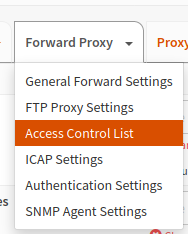
\includegraphics[width=0.2\textwidth]{Images/proxy/acl.PNG}
    \caption{Access control list}
    \label{opnsense:proxy_acl}
\end{figure}

\quesblock{\begin{enumerate}
    \item[37.] What are regular expressions?
    \item[38.] What is the difference between using \cmd{nrk.no} and \cmd{https://www.nrk.no} when filtering?
    \item[39.] How can you use a whitelist instead of a blacklist? 
\end{enumerate}}

\subsection{Category filtering}
Using a category list is an easy method to block a lot of URLs fast and easy. There are multiple services that provide such lists. One of them is Shalla, which is used in our example.

\setupblock{\begin{enumerate}
    \item Goto \cmd{Services --> Web-proxy --> Administration}
    \item Choose \cmd{Remote Access Control List}.
    \item Click on the + sign to add a new filter.
    \item Configure the following:
    \begin{enumerate}
        \item Make sure \cmd{Enabled} is checked.
        \item Set \cmd{Filename} to Shalla.
        \item Set \cmd{URL} to \url{https://www.shallalist.de/Downloads/shallalist.tar.gz}.
        \item And the \cmd{Description} to \cmd{Shalla}.
        \item Click save.
    \end{enumerate}
    \item Click \cmd{Download ACLs \& Apply}
\end{enumerate}}

\tipbox{The Shallalist that is downloaded contains over 70 different categories. To see them, click on the edit pencil sign and remove or add categories (figure \ref{opnsense:proxy_category}).}

\begin{figure}[h!]
    \centering
    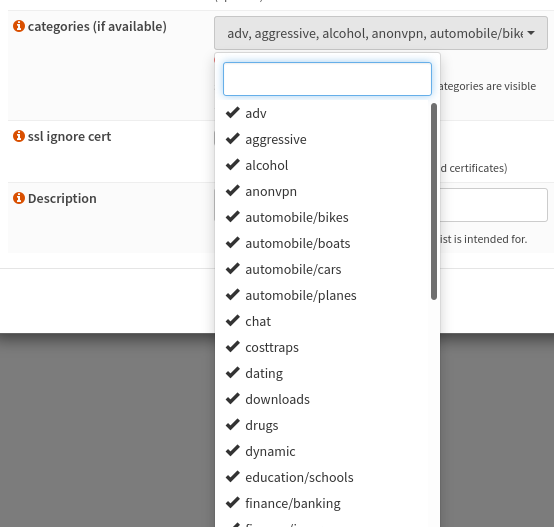
\includegraphics[width=0.5\textwidth]{Images/proxy/categories.PNG}
    \caption{Category blacklist}
    \label{opnsense:proxy_category}
\end{figure}

\subsubsection*{No proxy bypass}

First create two (2) firewall rules that block access without using proxy. Change the \cmd{Destinaiton port range} between \cmd{HTTP} and \cmd{HTTPS} for each of the rules created. The following configuration is only for \cmd{HTTP}:

\setupblock{\begin{enumerate}
    \item Go to \cmd{Firewall --> Rules --> LAN}.
    \item Change:
    \begin{enumerate}
        \item Set \cmd{Action} to \cmd{Block}.
        \item Set \cmd{Interface} to \cmd{LAN}.
        \item Set \cmd{Protocol} to \cmd{TCP/UDP}.
        \item Set \cmd{Source} to \cmd{LAN}.
        \item Set \cmd{Destination port range} to \cmd{HTTP}. Remember to change this to \cmd{HTTPS} for rule number two.
        \item Make a checkmark in the \cmd{Log} checkbox.
        \item Set \cmd{Category} to \cmd{Block Proxy Bypass}.
        \item Set \cmd{Descripion} to \cmd{Block http bypass}. Change this to \cmd{Block https bypass} for rule number two.
        \item Click \cmd{Save}.
    \end{enumerate}
    \item Go to \cmd{Services --> Web-proxy --> Administration}
    \item Choose \cmd{Forward Proxy}.
    \item Make a checkmark in the \cmd{Enable Transparent HTTP Proxy} check box.
\end{enumerate}}

\tipbox{Use the clone besides the pencil in the rule overview to clone the first rule and make the changes and save the new rule.}

\subsubsection*{Forward WAN traffic to proxy}

\setupblock{\begin{enumerate}
    \item Go to \cmd{Service --> Web Proxy}.
    \item Click the arrow beside \cmd{Forward Proxy} and choose \cmd{General Forward Settings}.
    \item Make a checkmark in the \cmd{Enable Transparent HTTP proxy} checkbox.
    \item Make a checkmark in the \cmd{Enable SSL inspection} checkbox.
    \item Click apply.
    \item Click on \cmd{Add a new firewall rule} in the help text for both \cmd{Enable Transparent HTTP Proxy} and \cmd{Enable SSL inspection}. If you do not see the help test, see \ref{get_help}. Accept the values and create the rule. Those rule will no be seen in the port forward section in NAT.
\end{enumerate}}

\begin{figure}[h!]
    \centering
    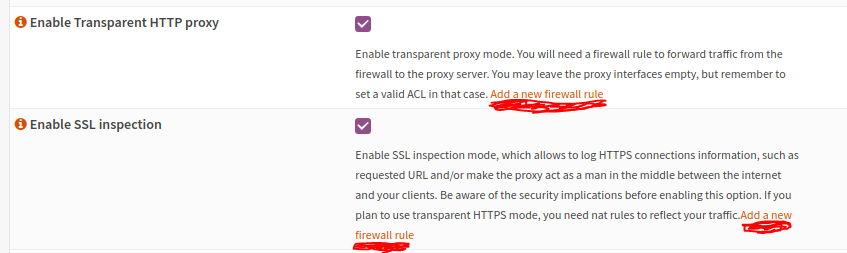
\includegraphics[width=0.6\textwidth]{Images/proxy/nat_rules.PNG}
    \caption{Creating NAT rules}
    \label{opnsense:proxy_ca_test}
\end{figure}


\quesblock{\begin{enumerate}
    \item[40.] Use some time and see if you can find another list that can be used.
    \item[41.] How can you test if the Shallalist is working? Just explain it, do not try to do it.
    \item[42.] How can you configure \opnsense\ to automatically update the rule list?
\end{enumerate}}

% Remove below?
%\subsection*{Authentication using proxy}
%Certificate or user:password

\subsection{Proxy logs}
For the proxy service there are three different logs that can be seen in the \cmd{Services --> web proxy}. \cmd{Cache log},\cmd{Access log}, and \cmd{Store log}.

\quesblock{\begin{enumerate}
    \item[43.] Explorer the three logs and explain what they log.
\end{enumerate}}

Learn more about Squid\footnote{\url{http://www.squid-cache.org/}} on their homepage.

\subsection{SSL inspection}
The firewall can act as a man in the middle and inspect packets that are encrypted. This is done using a proxy. When the firewall receives the packet, it decrypts it and inspects it. When the inspection is finished it encrypts the packet again. To make this work, the first step is to create a certificate that can be used to encrypt the traffic between the client and the firewall. This means that there are two connections per request. The first one between the client and the firewall, and the second one is between the firewall and the webserver.

\subsubsection{Create Certificate Authority} \label{create_ca}
The CA (Certificate Authority) needs to be either a self-signed root certificate or a certificate from an existing root CA. We are creating a self-signed one.
 
\setupblock{\begin{enumerate}
    \item Goto \cmd{System --> Trust --> Authorities}.
    \item Choose \cmd{Remote Access Control List}.
    \item Click on \cmd{Add}.
    \item Change the following:
    \begin{enumerate}
        \item Set \cmd{Descriptive name} to \cmd{ssl\_inspect.lab}.
        \item Set \cmd{Method} to \cmd{Create and internal Certificate Authority}.
        \item Set \cmd{Lifetime} to \cmd{3650}.
        \item Set \cmd{Country Code} to Norway.
        \item Set \cmd{State or Province} to \cmd{Agder}.
        \item Set \cmd{City} to \cmd{Kristiansand}.
        \item Set \cmd{Organization} to \cmd{Noroff}.
        \item Set \cmd{Email Address} to your Noroff student mail address.
        \item Set \cmd{Common Name} to \cmd{ssl\_inspect\_ca}.
    \end{enumerate}
    \item Click \cmd{Save}.
\end{enumerate}}

When the certificate is created, the next step is to export it. Click on the \cmd{Export CA cert} button. Save it on the client. This file will be used later when you configure your client.

\subsubsection{Firewall configuration}
Follow the configuration below to configure the firewall.

\setupblock{\begin{enumerate}
    \item Goto \cmd{Services --> Web-proxy --> Administration}.
    \item Goto \cmd{Forward Proxy}.
    \item Click the checkbox named \cmd{Enable SSL inspection}.
    \item Select to use the certificate we created in the previous configuration (\ref{create_ca}) in the \cmd{CA to use} dropdown menu.
    \item Click \cmd{Apply} to finish the server configuration.
\end{enumerate}}

\subsubsection{Client configuration}
The client configuration is done in Firefox on the Ubuntu client.

\setupblock{\begin{enumerate}
    \item Start Firefox and goto the \cmd{preferences} settings.
    \item Goto the \cmd{Privacy \& Security} tab.
    \item Click on \cmd{View Certificates}.
    \item Import the certificate created earlier (\ref{create_ca}).
    \item In the next window, click in the box beside \cmd{Trust this CA to identify websites}.
\end{enumerate}}

\subsubsection{Test}
Goto any website that is using \cmd{HTTPS} and checks who is verifying the connection. In this test example, \url{www.dagbladet.no} is used (figure \ref{opnsense:proxy_ca_test}). The connection, in this case, is verified by Noroff. This is in line with the information we used when configuring the CA earlier (\ref{create_ca}).

\begin{figure}[h!]
    \centering
    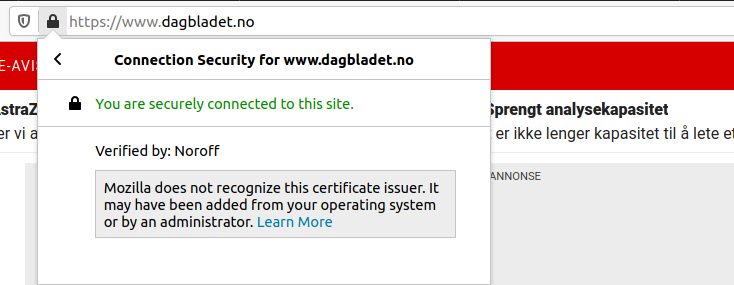
\includegraphics[width=0.5\textwidth]{Images/proxy/CA_test.PNG}
    \caption{CA test on \url{www.dagbladet.no}.}
    \label{opnsense:proxy_ca_test}
\end{figure}

%\subsection{SSL inspecttion using Transparent mode}

%\subsection{AntiVirus} % Unsure about this, since it is a plugin.
